\documentclass[10pt]{article}
\usepackage[margin=1in]{geometry} 
\usepackage{enumerate, xfrac, color, graphicx}
\usepackage{amsmath,amsthm,amssymb,amsfonts}
\usepackage{caption}
\usepackage{listings, courier}
\graphicspath{{figures}}
\usepackage{booktabs}
\newcommand{\N}{\mathbb{N}}
\newcommand{\Z}{\mathbb{Z}}
\lstset{breaklines=true, basicstyle=\small\ttfamily, language=R, backgroundcolor=\color{highlight}, stepnumber=5}

\definecolor{highlight}{RGB}{248,248,248}

\begin{document}
	\title{6.867 Problem Set 1}
	\maketitle

\subsubsection*{Linear Basis Function}

If we assume Gaussian errors,  $Y \sim N(X\theta, \sigma^2)$, then our maximum-likelihood estimator is equivalent to the OLS estimator. From Bishop, we know that
\begin{equation*}
	\hat{\theta}_{OLS}=\hat{\theta}_{ML}=(\Phi^T \Phi)^{-1}\Phi^T Y
\end{equation*}

where $\Phi$ denotes the polynomial basis expansion of $X$, for order $M$.

Below, we replicate Bishop's plots for $M$ = 0, 1, 3 and 10 using the aforementioned solution for the gradient.

\begin{figure}[ht]
	\centering
	\begin{minipage}[b]{.24\linewidth}
		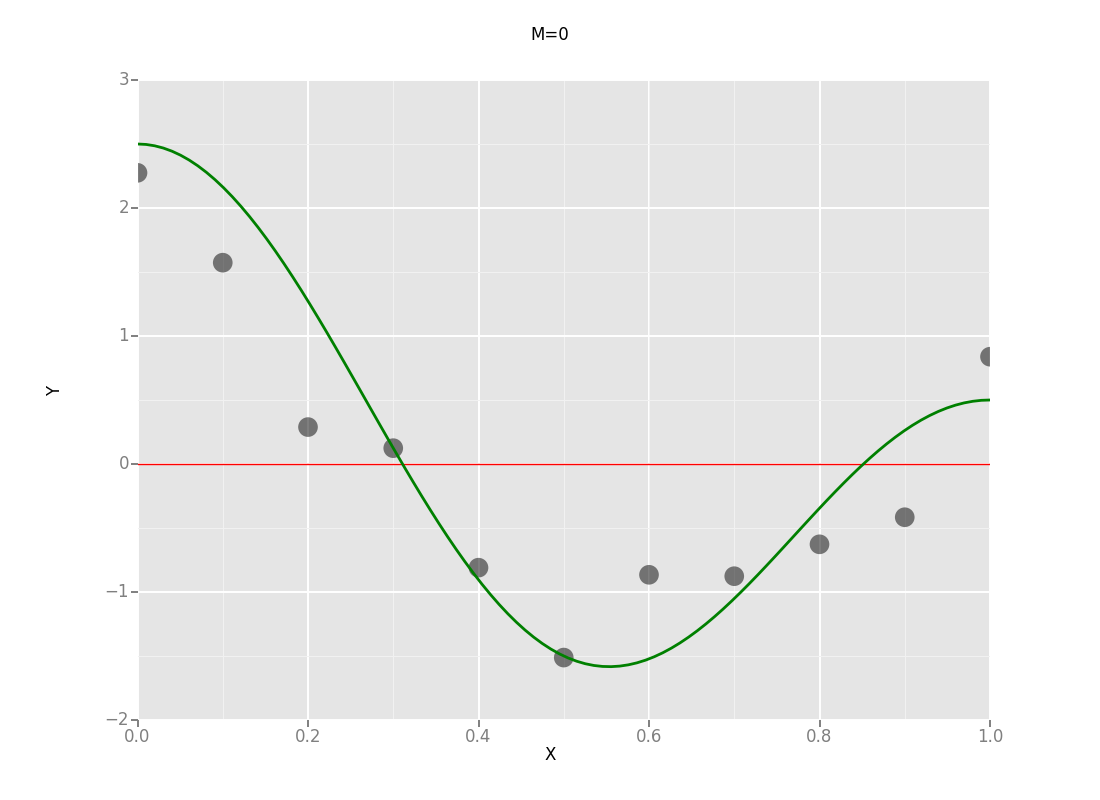
\includegraphics[width=1\linewidth, height=1.2in]{figures/M0.png}
		\caption*{$M=0$}
	\end{minipage}
	\begin{minipage}[b]{.24\linewidth}
		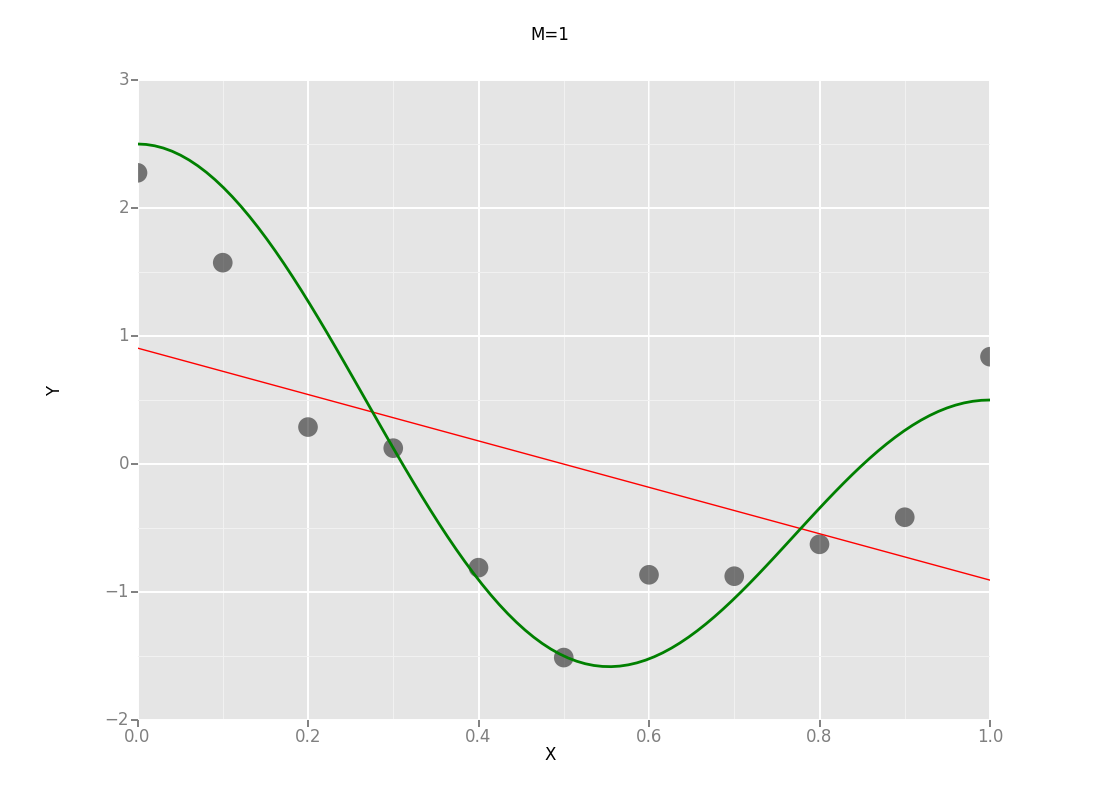
\includegraphics[width=1\linewidth, height=1.2in]{figures/M1.png}
			\caption*{$M=1$}
	\end{minipage}
	\begin{minipage}[b]{.24\linewidth}
		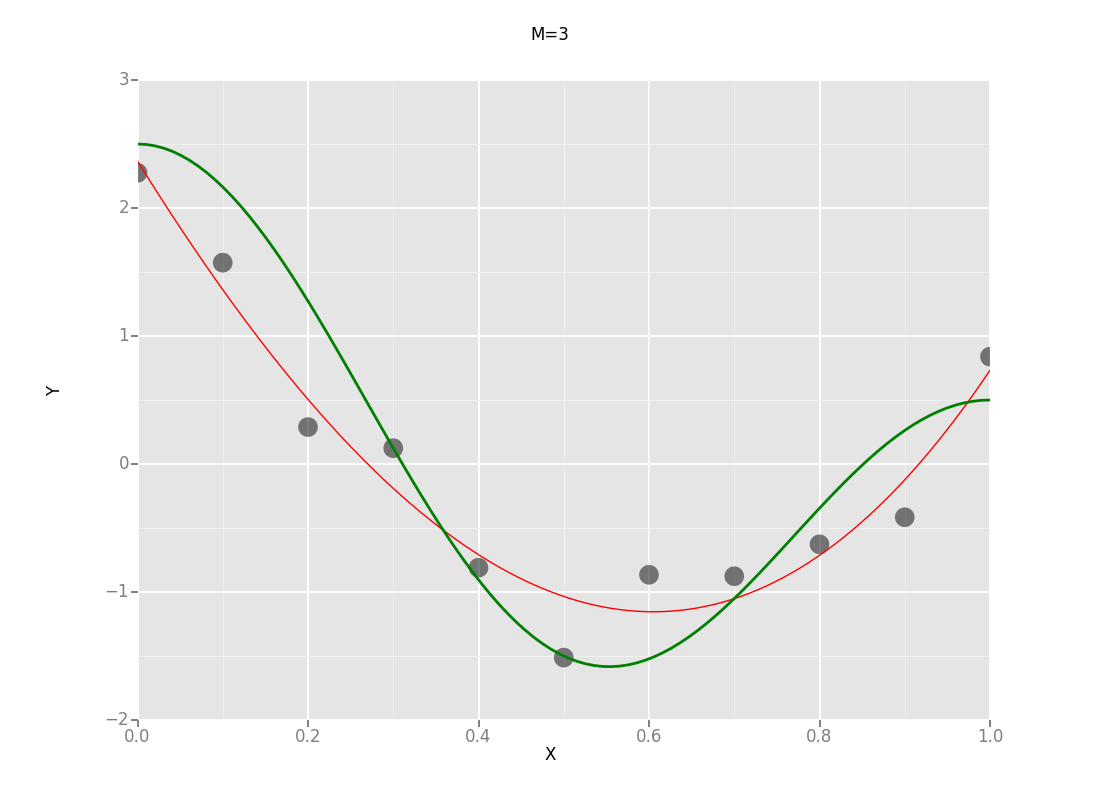
\includegraphics[width=1\linewidth, height=1.2in]{figures/M3.png}
		\caption*{$M=3$}
	\end{minipage}
	\begin{minipage}[b]{.24\linewidth}
		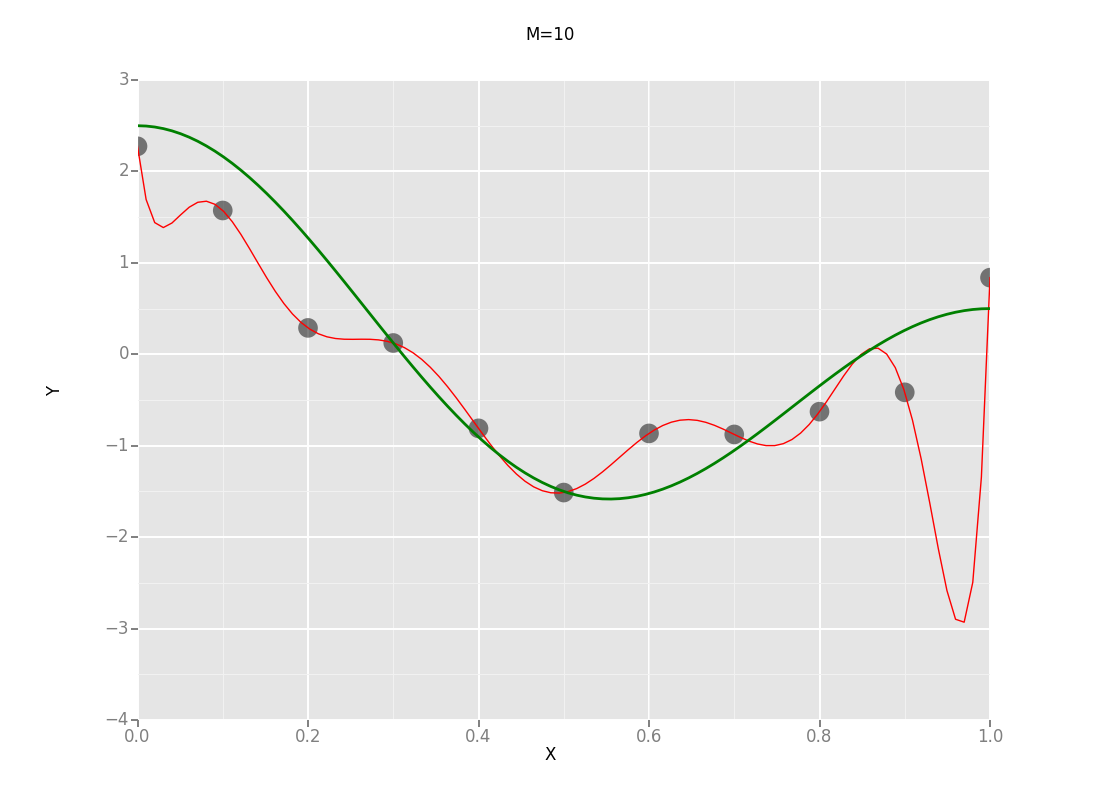
\includegraphics[width=1\linewidth, height=1.2in]{figures/M10.png}
		\caption*{$M=10$}
	\end{minipage}
	\caption{Plots of polynomials having various orders $M$, in red, fitted to the the observed points, green curve represents the function that actually generated the data.} 
\end{figure}


The sum of squared errors of a linear polynomial basis model is defined by: 
\begin{equation*}
	SSE=(\Phi \theta-Y)^T(\Phi \theta-Y)
\end{equation*}

with gradient 

\begin{equation*}
	\nabla SSE = 2\Phi^T(\Phi \theta-Y)
\end{equation*}
 which we verified with the central differences method for all values of $M$. We then compared the results of using Batch Gradient Descent and Stochastic Gradient Descent to find the optimal weights for different values of $M$. For BGD, learning rates between .02 and .06 converged for small values of $M$. For larger values of $M$,  learning rates had to be between .02 and .04 to get convergence.
 
 Using the Monro-Robbins learning schedule, where $k$ parameter impacts the steepness of the learning schedule, $\tau$ impacts the level of the learning rate, for SGD makes it difficult to directly compare learning rates between SGD and BGD, but, in general, SGD had to make many more iterations than BGD since it saw so much less data per iteration. Additionally, SGD needed a higher average learning rate to converge than BGD for all values of $M$.
 Reducing SGD's stopping criteria reduce the probability of stopping, regardless of whether the algorithm is stuck at a local minima or at the target. For this reason, reducing the stopping criterion is dangerous. Luckily, the decreasing learning schedule means that the weight does not fluctuate wildly near convergence, even if it doesn't meet the desired stability. 
 

To close our beautiful adventure with gradient descent, we tried to learn the optimal weights $\theta$ for the actual data generation process using different values of $M$. The results were very similar for all values of $M$. Below are the results for $M$=8.  The learned solution for all values of $M$ has lower MSE than the true weights,  we need to add a sparsity penalty to the loss function.

\begin{centering}
\begin{table}
\captionof{table}{2.4: Weights learned for Cosine Basic Expansion, M=8}

\begin{tabular}{lrr}
\toprule
{} &  Learned Weight &  True Weight \\
\midrule
w\_1 &            0.77 &          1.0 \\
w\_2 &            1.09 &          1.5 \\
w\_3 &            0.10 &          0.0 \\
w\_4 &            0.14 &          0.0 \\
w\_5 &           -0.05 &          0.0 \\
w\_6 &            0.36 &          0.0 \\
w\_7 &            0.01 &          0.0 \\
w\_8 &            0.02 &          0.0 \\
\bottomrule
\end{tabular}

\end{table}
\end{centering}

\subsubsection*{Ridge Regression}

Given the problems we faced for high values of M when learning the Cosine basis function, we will now add a regularization term  $\lambda$ to our loss function to push coefficients towards 0 and avoid overfitting. 

Let's now see how regression behaves when we impose a regularization term. The regularization term,, serves to make sure we don't overfit to our training data. 

The closed form solution for Ridge from Bishop equation 3.27
\begin{equation}
\hat{\theta} = (\mathbf{X}^T\mathbf{X} + \lambda \mathbf{I})^{-1}\mathbf{X}^t\mathbf{y}
\end{equation}

\noindent where $\mathbf{X}$ is the feature matrix after the polynomial basis transformation and  $y$ are the targets, and $\hat{\theta}$ are the feature coefficients. $\lambda$ is a regularization parameter --  a higher lambda will penalize the model more for having large feature weights, a lower model will penalize the model less. With $\lambda =0$ the solution is the same as that or Ordinary Least Squares.

For data we were given a training set of 13 observations, a testing set of 10 observations and a validation set of 22 observations. The algorithm for optimizing hyperparameters was to 1) search for the best combination of $M$ and $\lambda$ by training the model on the training data and testing it on the validation set. 2) given the optimal  $M$ and $\lambda$  (based on validation set performance), use the corresponding $\hat{\theta}$ to attempt to predict values of $\mathbf{y}$ for the test data, and measure the Mean Squared Error of our predictions. We also experimented with training on flipping the test and train dataset to check whether our labeling was robust to the outlier in dataset B. The following table shows the results of that procedure on a search space of  $\lambda$ in $[0, .1, .5, 1, 3,5,10, 12, 100, 200, 1000, 10000]$ and $M$  between 1 and 5. For both train/test splits, the optimal $M$ is 2, whereas the optimal $\lambda$s are in the same range. 

As we expect, higher values of M and lower values of L lead to a near perfect in-sample fit to the data. However, the validation set enforces a lower M. Interestingly, however, since dataset A and the validation set are fairly well behaved (strong relationship between X and Y, no outliers), regularization does not help on the validation set. and a model with M=2 and no regularization performs well. All the models, including those with higher $\lambda$, perform considerably worse on the test set.

When we train on dataset B, which has a significant outlier, however, regularization reduces Validation and test MSE. By pushing coefficients towards 0, the model is less impacted by the outlier and therefore does a better a job of predicting the test and validation sets. In this procedure, models with  $\lambda = 0.5, M=3$ performed the best on the validation set. As the below table shows, however, more regularization would have helped. The best parameters for the test validation set  were  $\lambda = 0.5, M=3$  though $\lambda = 5, M=1$ would have performed better on the test set.  Since regularization prevents over-fitting, it adds more value when there are outliers in the training data. 


\begin{tabular}{llrrr}

  &     &  Train MSE &  Validation MSE &  Test MSE \\
M & L &            &                 &           \\

1 & 0.0 &       1.44 &            1.60 &      1.82 \\
  & 0.5 &       1.44 &            1.52 &      1.71 \\
  & 5.0 &       1.72 &            1.33 &      1.36 \\
3 & 0.0 &       0.98 &            1.38 &      3.76 \\
  & 0.5 &       1.00 &            1.28 &      3.16 \\
  & 5.0 &       1.32 &            1.80 &      2.58 \\

\end{tabular}
\end{document}
